\section{Introduction}
The interest for application-specific hardware is increasing, as they provide a feasible solution to allow both energy savings and performance gain over their counterparts~\cite{hameed2010understanding}, thus matching current application demands.
%ADDCITATION ((2013). The End of Dennard Scaling. Accessed: Feb. 2013. [Online].
%Available: https://cartesianproduct.wordpress.com/2013/04/15/the-endof-dennard-scaling/
%[3] H. Esmaeilzadeh, E. Blem, R. S. Amant, K. Sankaralingam, and
%D. Burger, “Dark silicon and the end of multicore scaling,” in Proc.
%38th Annu. Int. Symp. Comput. Archit. (ISCA), Jun. 2011, pp. 365–376.}
It has been shown that the memory system (both on-chip and off-chip) has become a dominant factor affecting the overall performance~\cite{williams2009roofline}, power consumption~\cite{dayarathna2015data}, and silicon area usage~\cite{oh2009analytical}. Since the memory system and the processing system are strongly \textit{interdependent}, they should be \textit{co-designed}. This is especially important for emerging memory technologies, such as MRAM, eDRAM, PCM, RRAM~\cite{mem2016}, that have higher integration density and lower power than SRAM, but features different latency for read and write operations.

%
%BibTeX | EndNote | ACM Ref
%@inproceedings{Hameed:2010:USI:1815961.1815968,
% author = {Hameed, Rehan and Qadeer, Wajahat and Wachs, Megan and Azizi, Omid and Solomatnikov, Alex and Lee, Benjamin C. and Richardson, Stephen and Kozyrakis, Christos and Horowitz, Mark},
% title = {Understanding Sources of Inefficiency in General-purpose Chips},
% booktitle = {Proceedings of the 37th Annual International Symposium on Computer Architecture},
% series = {ISCA '10},
% year = {2010},
% isbn = {978-1-4503-0053-7},
% location = {Saint-Malo, France},
% pages = {37--47},
% numpages = {11},
% url = {http://doi.acm.org/10.1145/1815961.1815968},
% doi = {10.1145/1815961.1815968},
% acmid = {1815968},
% publisher = {ACM},
% address = {New York, NY, USA},
% keywords = {ASIC, chip multiprocessor, customization, energy efficiency, h.264, high performance, tensilica},
%} 

CAD tools~\cite{synopsystool,tensilica,codasiptool} are available to help with the increasing complexity of custom processor design. However, selecting an optimal hardware architecture, taking into account the various trade-offs in latency, power consumption, and area usage remains a challenging task. State-of-the-art design flows for custom-processor design-space exploration focus on processor architecture optimization~\cite{Meloni2012,EusseSAMOS2014,Jozwiak2013,Karuri2009}, and do not include the memory system, as illustrated in Figure~\ref{fig:intro}. Co-optimization of the processor and the memory system (including emerging memories) is typically done by co-simulation and by optimization the cache replacement policy~\cite{4798259,7092595,6271803,Mittal13f}. 
%Papers to cite for CDFG generation and Application Specific High LSynthesis~\cite{Coussy:2008:HSA:1457713,Kato2008}.
One exception are the emerging spatial architectures~\cite{7284058,8686088}, which distribute the program memory and processing elements to achieve maximum performance; however, they use rigid interconnect topologies to allow flexible communication between processing elements leading to larger area and power utilization.

\begin{figure}[ht]
    \centering
    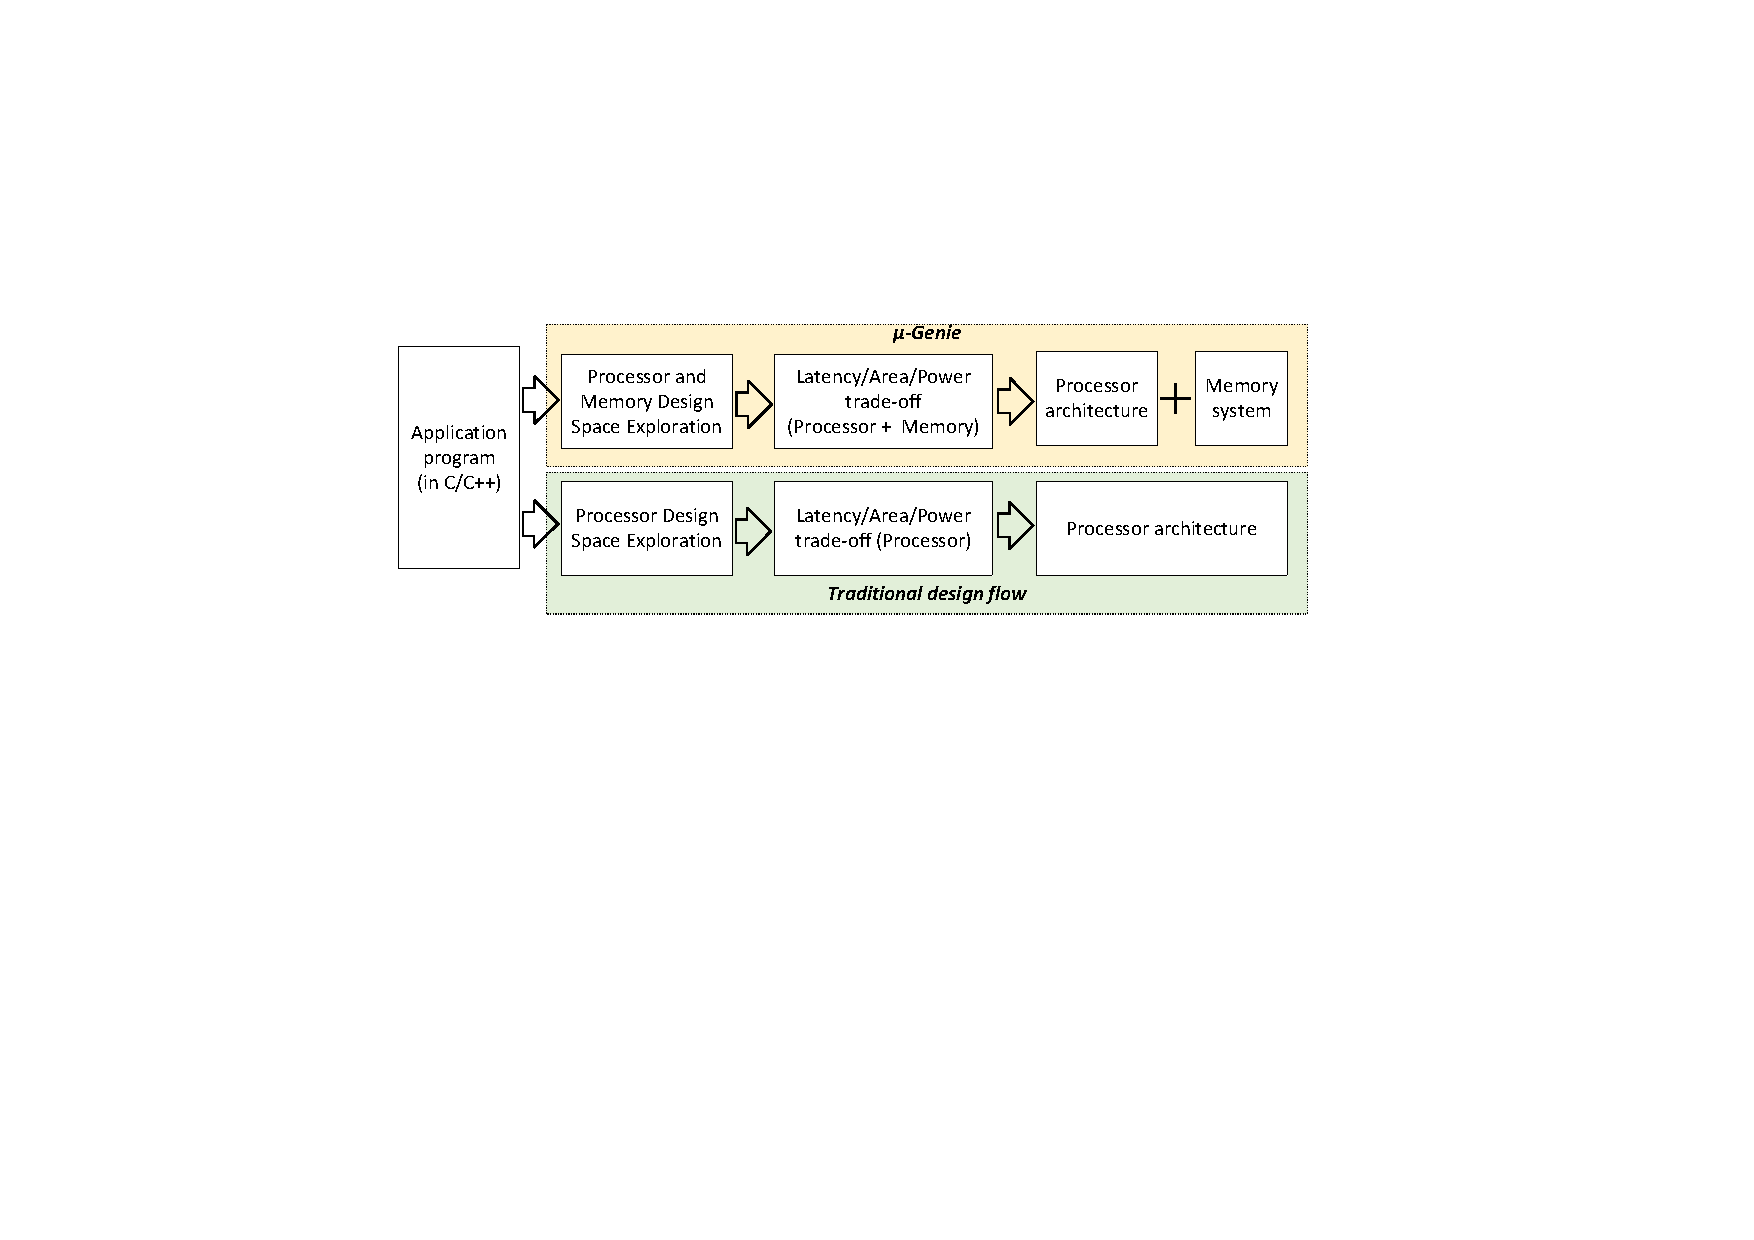
\includegraphics[clip, trim=6cm 10.5cm 6.4cm 5.2cm, width=1.0\linewidth]{images/intro_figure.pdf} %[left down right up ] 
    \caption{Difference between state-of-the-art and the proposed \frameworkname~design flows for custom processor architecture design.}
    \label{fig:intro}
\end{figure}
In this work, we propose \frameworkname, an automated framework for memory-aware custom processor architecture design-space exploration and provide different tradeoffs (\ref{sec:framework}), as shown in Figure~\ref{fig:intro}. The framework supports different kinds of memory technologies and the configuration levels of memory, clock frequency, read/write latency and data width. Moreover, using spatial architectural templates (\ref{sec:arch_template}), \frameworkname~can generate ready-to-use designs for the co-designed processors. These designs can be configured at design-time (based on the trade-off from the framework) and allow a faster prototyping of an application-specific hardware. Finally, to demonstrate the capabilities of \frameworkname, we propose two case-studies analysing custom-processor designs using state-of-the-art MRAM and SRAM for the memory system (\ref{sec:case_studies}).
 
\frameworkname~enables design space exploration for application-specific custom-processors beyond the current state-of-the-art solutions, even enabling a first comparison between different memory technologies, like MRAM and SRAM.

%In this work we present \frameworkname, a framework that allows to compare design choices and perform automatic system level design and implementation. We propose a novel memory-driven approach for application-specific hardware design starting from two observations. First, the memory system and the processing system are \textit{interdependent} and therefore they should be \textit{co-designed}. Second, the \textit{data dependencies} of the fixed application impose constaints on the design of both memory and processing systems. Hence, our approach starts from the analysis of an input application and codesigns memory and custom processor, shown in Figure~\ref{fig:intro}. 



